\chapter{Previous Work}
\section{C-LexRank Algorithm}
In this section we describe C-LexRank as a method to extract citing sentences that cover
a diverse set of factoids. The method works by modeling the set of citations as a network
of sentences and identifying communities of sentences that cover similar factoids. Once a
good division of sentences is made, we extract salient sentences from different communities.
Figure 1 illustrates a representative example that depicts C-LexRank$'$s process.

\begin{figure}[!htbp]
\centering
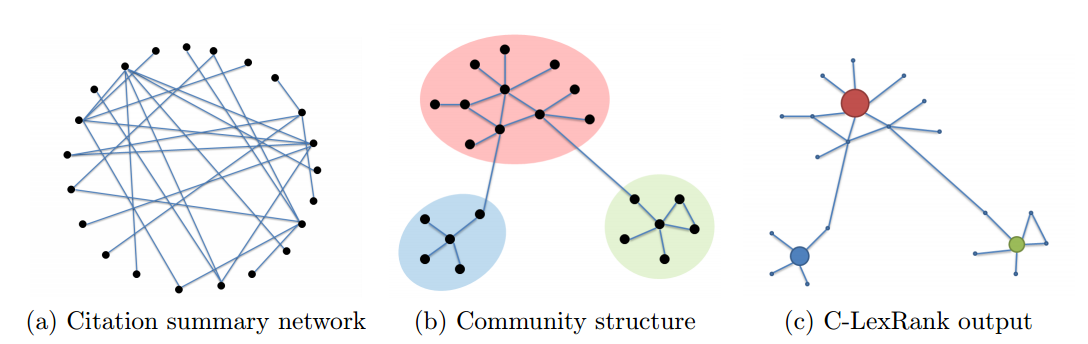
\includegraphics[width=15cm]{LexRank.png}
\caption{ The C-LexRank method extracts citing sentences that cover a diverse set of factoids.
The citation summary network in (a) models the set of sentences that cite
a specific paper, where vertices represent citing sentences and (weighted) edges
show the degree of semantic relatedness between vertex pairs. The community
structure in (b) corresponds to clustered sets of representative sentences extracted
from citation sentences. The C-LexRank output in (c) corresponds to the candidate
sentences from different clusters that are used for building a summary}
\label{cLexRank}
\end{figure}

\subsection{ Citation Summary Network}
In the first step (as shown in Figure 1 (a)), we model the set of sentences that cite a specific
paper with a network in which vertices represent citing sentences and undirected weighted
edges show the degree of semantic relatedness between vertex pairs, normally quantified
by a similarity measure. We refer to this network as the Citation Summary Network of
an article. The similarity function should ideally assign high scores to sentence pairs that
have the same factoids, and should assign low scores to sentences that talk about different
contributions of the target paper.
Previously, Qazvinian and Radev (2008) examined 7 different similarity measures including
TF-IDF with various IDF databases, longest common sub-sequence, generation
probability (Erkan, 2006), and the Levenstein distance on a training set of citations. They
showed that the cosine similarity measure that employs TF-IDF vectors assigns higher similarities
to pairs that contain the same factoids. Following Qazvinian and Radev (2008), we
use the cosine similarity between TF-IDF vector models that employ a general IDF corpus to construct the citation summary network of each article.

\begin{figure}[!htbp]
\centering
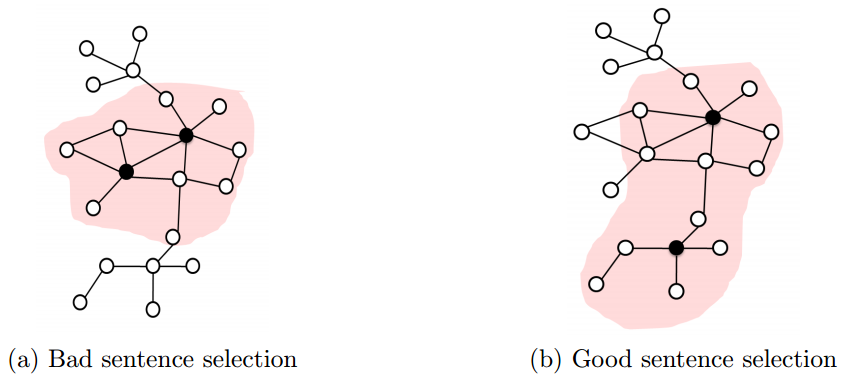
\includegraphics[width=15cm]{fig2lexrank.png}
\caption{ The C-LexRank method extracts citing sentences that cover a diverse set of factoids.
The citation summary network in (a) models the set of sentences that cite
a specific paper, where vertices represent citing sentences and (weighted) edges
show the degree of semantic relatedness between vertex pairs. The community
structure in (b) corresponds to clustered sets of representative sentences extracted
from citation sentences. The C-LexRank output in (c) corresponds to the candidate
sentences from different clusters that are used for building a summary}
\label{cLexRank2}
\end{figure}

\subsection{Community Structure}
In the second step (as shown in Figure 1 (b)), we extract vertex communities from the
citation summary network to generate summaries. We generate summaries by extracting
representative sentences from the citation summary network. Intuitively, a good summary
should include sentences that represent different contributions of a paper. Therefore, a good
sentence selection from the citation summary network will include vertices that are similar
to many other vertices and which are not very similar to each other. On the other hand,
a bad selection would include sentences that are only representing a small set of vertices
in the graph. This is very similar to the concept of maximizing social influence in social
networks (Kempe, Kleinberg, \& Eva Tardos, 2003). Figure 2 shows an example in which the ´
selected two vertices in the citation summary networks represent a small subset of vertices
(left) and a larger subset of vertices (right). In our work we try to select vertices that maximize the size of the set of vertices that they represent. We achieve this by detecting
different vertex communities in the citation summary network. In order to find vertex communities and thus a good sentence selection, we exploit the
small-world property of citation summary networks. A network is called \textit{small-world}, if
most of its vertices are not neighbors of each other, but can be reached from one another
by a small number of steps (Watts \& Strogatz, 1998). Recent research has shown that a
wide range of natural graphs such as biological networks (Ravasz, Somera, Mongru, Oltvai,
\& Barab´asi, 2002), food webs (Montoya \& Sol´e, 2002), brain neurons (Bassett \& Bullmore,
2006) and human languages (Ferrer i Cancho \& Sol´e, 2001) exhibit the small-world property.
This common characteristic can be detected using two basic statistical properties: the
clustering coefficient C, and the average shortest path length \textit{l}. The clustering coefficient
of a graph measures the number of closed triangles in the graph. It describes how likely
it is that two neighbors of a vertex are connected (Newman, 2003). Watts and Strogatz
(1998) define the clustering coefficient as the average of the local clustering values for each
vertex.
\begin{center}
C = $\frac{\sum_{i=1}^{n} c_i}{n}$
\end{center}


The local clustering coefficient $C_i$ for the $i_{th}$ vertex is the number of triangles connected
to vertex i divided by the total possible number of triangles connected to vertex i. Watts
and Strogatz (1998) show that small-world networks are highly clustered and obtain relatively
short paths (i.e., \textit{l} is small). Previous work (Qazvinian \& Radev, 2011a) shows that
citation summary networks are highly clustered. These networks have small shortest paths
and obtain clustering coefficient values that are significantly larger than random networks.
Moreover, Qazvinian and Radev suggest that this is because of a community structure, where each community is composed of a set of highly connected vertices with a small number
of edges that fall between communities.

\begin{figure}[!htbp]
\centering
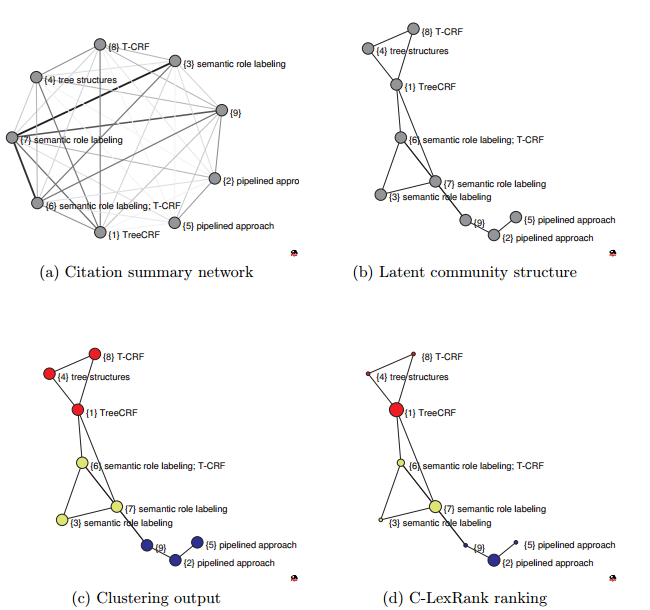
\includegraphics[width=15cm]{fig3lexRank.png}
\caption{ The C-LexRank method extracts citing sentences that cover a diverse set of factoids.
The citation summary network in (a) models the set of sentences that cite
a specific paper, where vertices represent citing sentences and (weighted) edges
show the degree of semantic relatedness between vertex pairs. The community
structure in (b) corresponds to clustered sets of representative sentences extracted
from citation sentences. The C-LexRank output in (c) corresponds to the candidate
sentences from different clusters that are used for building a summary}
\label{cLexRank}
\end{figure}


\subsection{Ranking}

The third step of the C-LexRank process (as shown in Figure 1 (c)) is applied after the
graph is clustered and the communities are formed. To produce the C-LexRank output,we extract sentences from different clusters to build a summary. We start with the largest
cluster and extract sentences using LexRank (Erkan \& Radev, 2004) within each cluster. In
other words, for each cluster Ωi we made a lexical network of the sentences in that cluster
(Ni). Using LexRank we can find the most central sentences in Ni as salient sentences of Ωi
to include in the main summary. We choose, for each cluster Ωi, the most salient sentence
of Ωi, and if we have not reached the summary length limit, we do that for the second most
salient sentences of each cluster, and so on. The cluster selection is in order of decreasing
size. Figure 3 (d) shows Cohn and Blunsom’s (2005) citation summary network, in which
each vertex is plotted with a size proportional to its LexRank value within its cluster. This
figure shows how C-LexRank emphasizes on selecting a diverse set of sentences covering a
diverse set of factoids.
Previously, we mentioned that factoids with higher weights appear in a greater number
of sentences, and clustering aims to cluster such fact-sharing sentences in the same communities.
Thus, starting with the largest community is important to ensure that the system
summary first covers the factoids that are more frequently mentioned in other citation
sentences and thus are more important.
The last sentence in the example in Table 2 is as follows. “We use CRFs as our models
for both tasks (Cohn \& Blunsom, 2005).” This sentence shows that a citation may not
cover any contributions of the target paper. Such sentences are assigned by the community
detection algorithm in C-LexRank to clusters to which they are semantically most similar.
The intuition behind employing LexRank within each cluster is to try to avoid extracting
such sentences for the summary, since LexRank within a cluster enforces extracting the most
central sentence in that cluster. In order to verify this, we also try a variant of C-LexRank
in which we do not select sentences from clusters based on their salience in the cluster, but
rather in a round-robin fashion, in which all the sentences within a cluster are equally likely
to be selected. We call this variant C-RR.

\pagebreak
\section{Evaluation scheme}

To evaluate our system, we use the pyramid evaluation method (Nenkova \& Passonneau,
2004). Each factoid in the citations to a paper corresponds to a summary content unit
(SCU) in (Nenkova \& Passonneau, 2004).
The score given by the pyramid method for a summary is the ratio of the sum of the
weights of its factoids to the sum of the weights of an optimal summary. This score ranges
from 0 to 1, and high scores show the summary content contains more heavily weighted
factoids. If a factoid appears in more citation sentences than another factoid, it is more
important, and thus should be assigned a higher weight. To weight the factoids we build a
pyramid, and each factoid falls in a tier. Each tier shows the number of sentences a factoid
appears in. Thus, the number of tiers in the pyramid is equal to the citation summary size.
If a factoid appears in more sentences, it falls in a higher tier.

So, if the factoid $f_i$ appears $\lvert f_i \rvert$
 times in the citation summary it is assigned to the tier $T_{\lvert f i\rvert}$.
 
 The pyramid score formula that we use is computed as follows. Suppose the pyramid
has n tiers, $T_i$
, where tier $T_n$ on top and $T_1$ on the bottom. The weight of the factoids in
tier $T_i$ will be i (i.e. they appeared in i sentences). If $\lvert T_i
\rvert$ denotes the number of factoids in
tier $T_i$
, and $D_i$
is the number of factoids in the summary that appear in $T_i$
, then the total
factoid weight for the summary is as follows.

\begin{center}
    D = $\sum_{i=1}^{n} i \times D_i$
\end{center}

Additionally, the optimal pyramid score for a summary with X factoids, is

\begin{center}
\textit{Max} = $\sum_{i=j+1}^{n} i \times \lvert T \rvert  + j \times (X - \sum_{i=j+1}^{n}\lvert T \rvert)$
\end{center}
where $j = max_i(\sum_{t=1}^{n}\lvert T_t \rvert \geq X)$ ). Subsequently, the pyramid score for a summary is calculated
as follows.

\begin{center}
P = $\frac{D}{Max}$
\end{center}
